\subsection{NOT}
    The NOT gate, also known as an inverter, is the simplest type of logic gate. 
    The circuitry consists of a single transistor along with some associated resistors and it is shown in Figure \ref{fig:NOT_circuit}. \\
    It is equivalent to the logical negation operator ($\neg$) in mathematical logic, as its primary function is to output the logical complement of the input.
    Its operation can be algebraically represented as $\text{NOT}(A) = \overline{A}$, while its analytical representation is $f(A)=1-A$, where $A$ is the input signal. \\
    When the input is high (1), the transistor is turned on, creating a low output (0). 
    Conversely, when the input is low (0), the transistor is off, resulting in a high output (1).
    This behavior is consistent with the NOT gate's truth table shown in Table \ref{tab:NOT_table}. \\
    The symbol for the NOT gate, in Figure \ref{fig:NOT_sym}, consists of a triangle with a circle at its output.

    \begin{figure}[H]
        \begin{minipage}{0.5\textwidth}
            \centering
            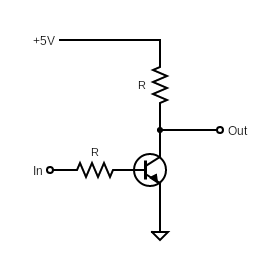
\includegraphics[width=0.8\textwidth]{figures/circuits/NOT.png}
            \captionof{figure}{NOT schematic circuit.}
            \label{fig:NOT_circuit} 
        \end{minipage}
        \begin{minipage}{0.5\textwidth}
            \centering
            \captionof{table}{NOT truth table.}
            \begin{tabular}{|c|c|}
                \hline
                Input & Output \\
                \hline
                0 & 1 \\
                1 & 0 \\
                \hline
            \end{tabular}
            \label{tab:NOT_table}
        \end{minipage}
    \end{figure}

    \begin{figure}[H]
	    \centering
	    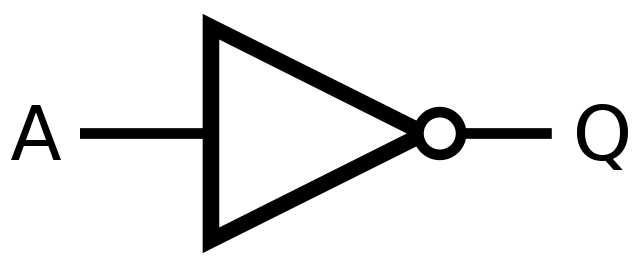
\includegraphics[width=0.3\textwidth]{figures/symbols/NOT.png}
	    \caption{NOT symbol.}
	    \label{fig:NOT_sym} 
	\end{figure}

    % \vspace{1.2cm}